%
\documentclass[12pt,a4paper]{article}

\usepackage[utf8]{inputenc}
\usepackage[usenames,dvipsnames]{xcolor}
\usepackage{graphicx}
\usepackage[margin=1in]{geometry}
\usepackage[]{natbib}
\usepackage[]{sidecap}
\usepackage{setspace}
\usepackage{defs}
\usepackage{lastpage}
\usepackage{fancyhdr}
\usepackage{pdfpages}
\usepackage{enumitem}

\usepackage{libertine}
\usepackage[T1]{fontenc}

\usepackage[pdftex]{hyperref}
\hypersetup {
    bookmarks=true,                    % show bookmarks bar in pdf reader
    pdftitle={Research Proposal - 2016 VR Etableringsbidrag},                   
    pdfauthor={Gregory A. Feiden},     % set pdf author
    pdfsubject={}, % pdf subject
    colorlinks=true,                   % false = box link, true = colored links
    linkcolor=black,                   % color of internal links
    citecolor=black,                    % color of citations
    urlcolor=NavyBlue                      % external url color
}
\urlstyle{same}

\citestyle{aa}
\bibliographystyle{mn}

\pagestyle{fancy}
\fancyhead[L]{Gregory Feiden -- Personal Number -- Research Plan}
\fancyhead[R]{\thepage\ of\ \pageref{LastPage}}
\fancyfoot[C]{}
\renewcommand{\headrulewidth}{0.0pt}

\fancypagestyle{plain}{
    \fancyhf{}
    \fancyfoot[C]{\thepage\ of\ \pageref{LastPage}}
    \renewcommand{\headrulewidth}{0.0pt}
    \renewcommand{\footrulewidth}{0.0pt}
}

\setlength{\parindent}{0pt}
\setlength{\parskip}{0.5\baselineskip}
\newenvironment{myindentpar}[1]%
 {\begin{list}{}%
         {\setlength{\leftmargin}{#1}}%
         \item[]%
 }
 {\end{list}}

\begin{document}

\begin{center}
	{\bf {\LARGE Ages of Young Stars and the Evolution of 
	
	Dynamo-Generated Stellar Magnetic Fields}} 
\end{center}

Astrophysical phenomena generally occur over time periods inaccessible to even the most patient human. Typical timescales range from thousands to billions of years. Nevertheless, time dependence is a vital component in our understanding astrophysical processes. 
%To overcome the difficulties 
Instead of monitoring a single system over time, astronomers gain insight into the time dependence of astrophysical phenomena by considering an ensemble of systems at different ages. Individual systems provide snapshots in time and a chronological ordering produces a stop-motion film of various processes across cosmic time. Accurate absolute ages are therefore the most sought after astrophysical quantities. This is particularly true for young systems, where ages provide critical constraints on the formation of stars, planets, and objects in-between. However, despite their importance, accurate ages for young systems remain elusive.

\vspace{\baselineskip}

{\bf \large Purpose and Aims}

\clearpage

{\bf \large Survey of the Field}
\begin{itemize}
	\item Age-dating problems for young stars. (i.e., model inconsistencies)
	\item Identification / inclusion of magnetic fields in models. (D'Antona, MacDonald, Feiden)
	\item Magnetic field observations. (e.g., MDI, ZDI)
	\item Open questions.
\end{itemize}

\begin{figure}
	\centering
	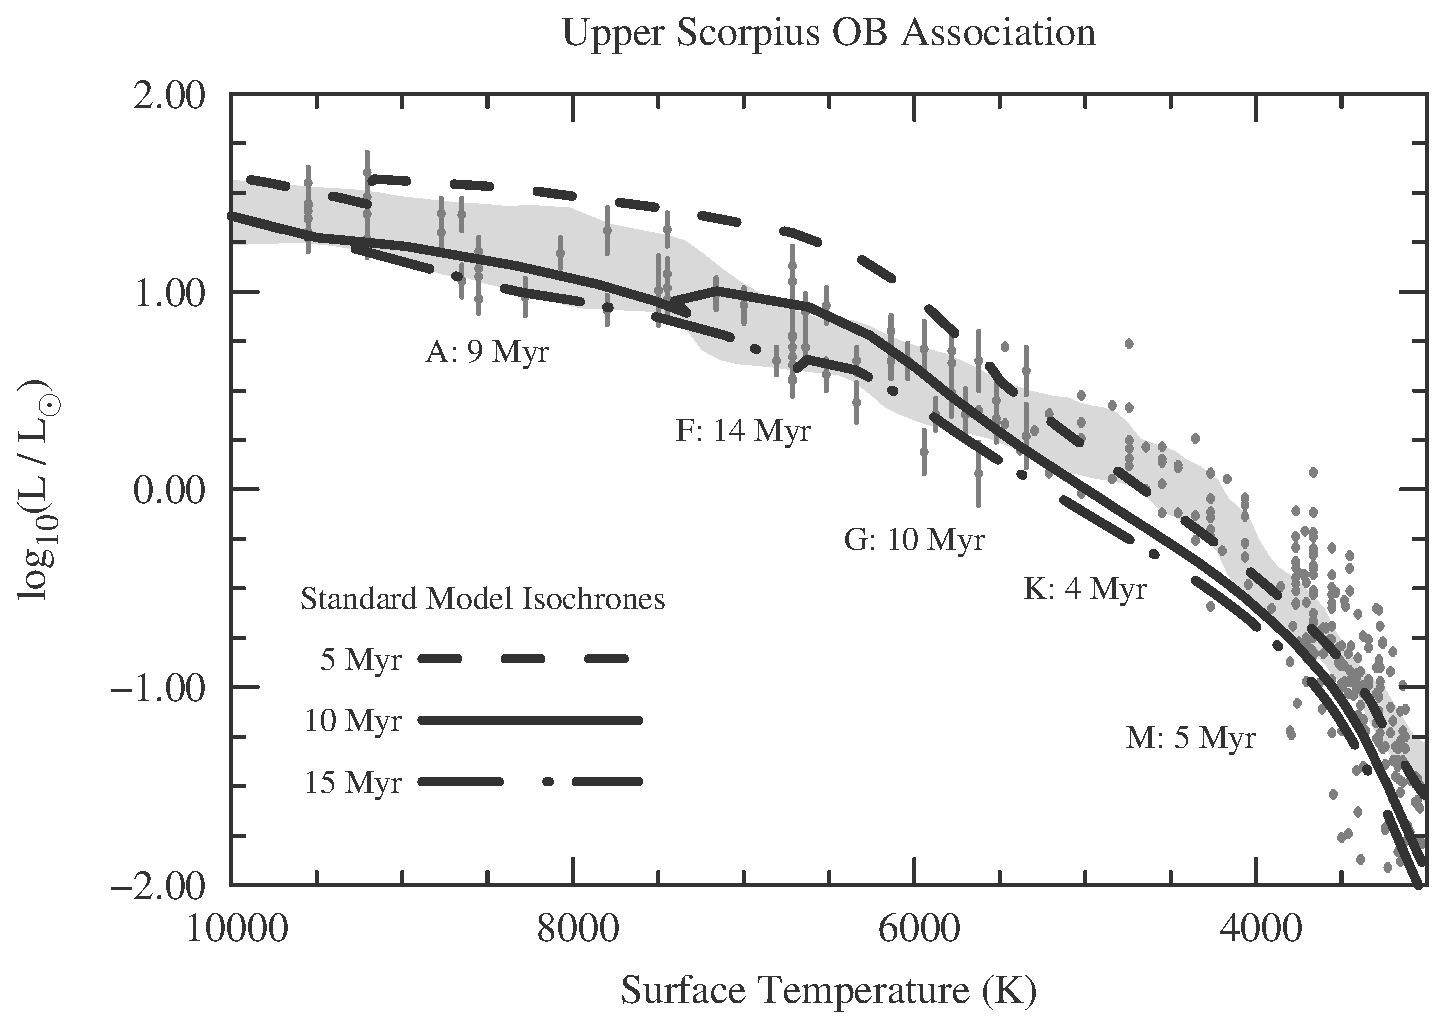
\includegraphics[width=0.75\linewidth]{./fig/USco_Age_Problems.eps}
	\caption{Caption.}
	\label{fig:probs}
\end{figure}

\begin{figure}
	\centering
	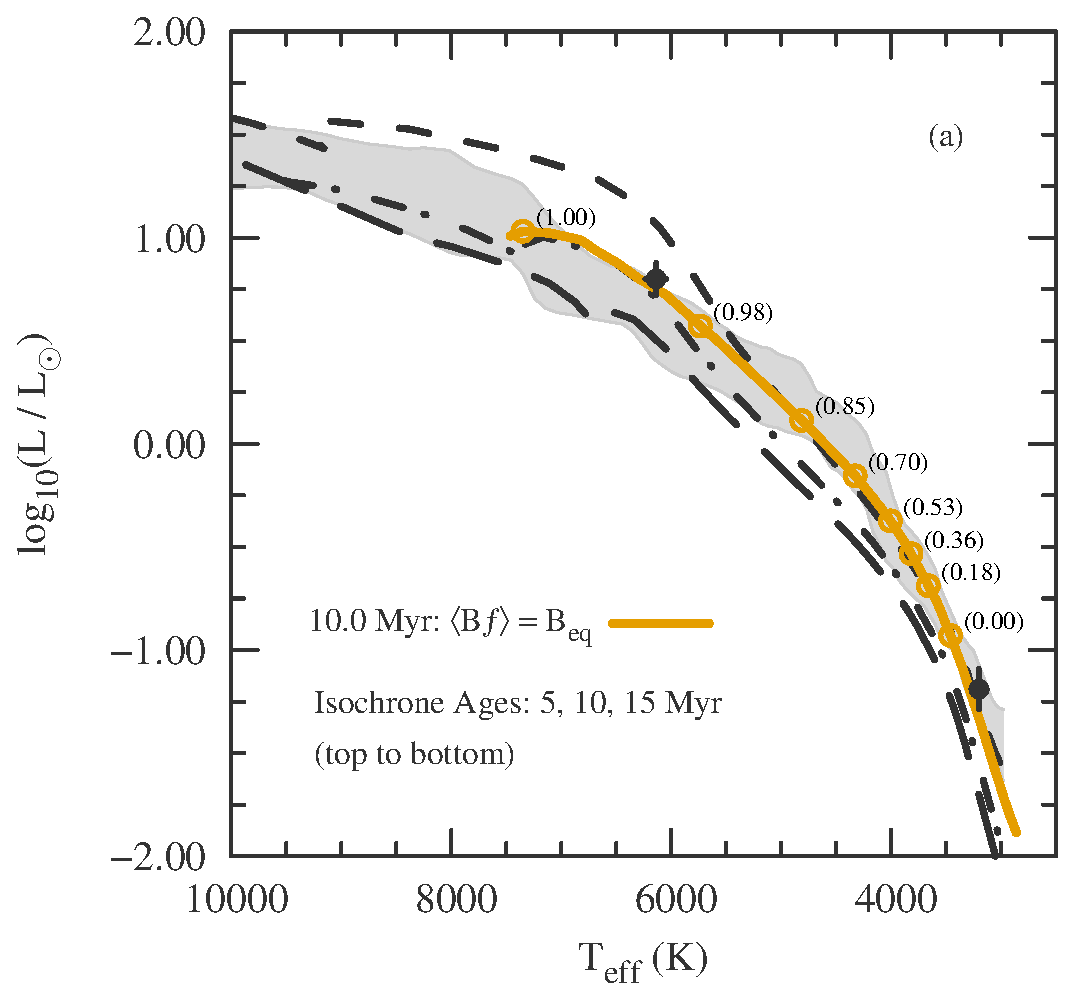
\includegraphics[width=0.45\linewidth]{./fig/USco_HR_diagram.eps} \qquad
	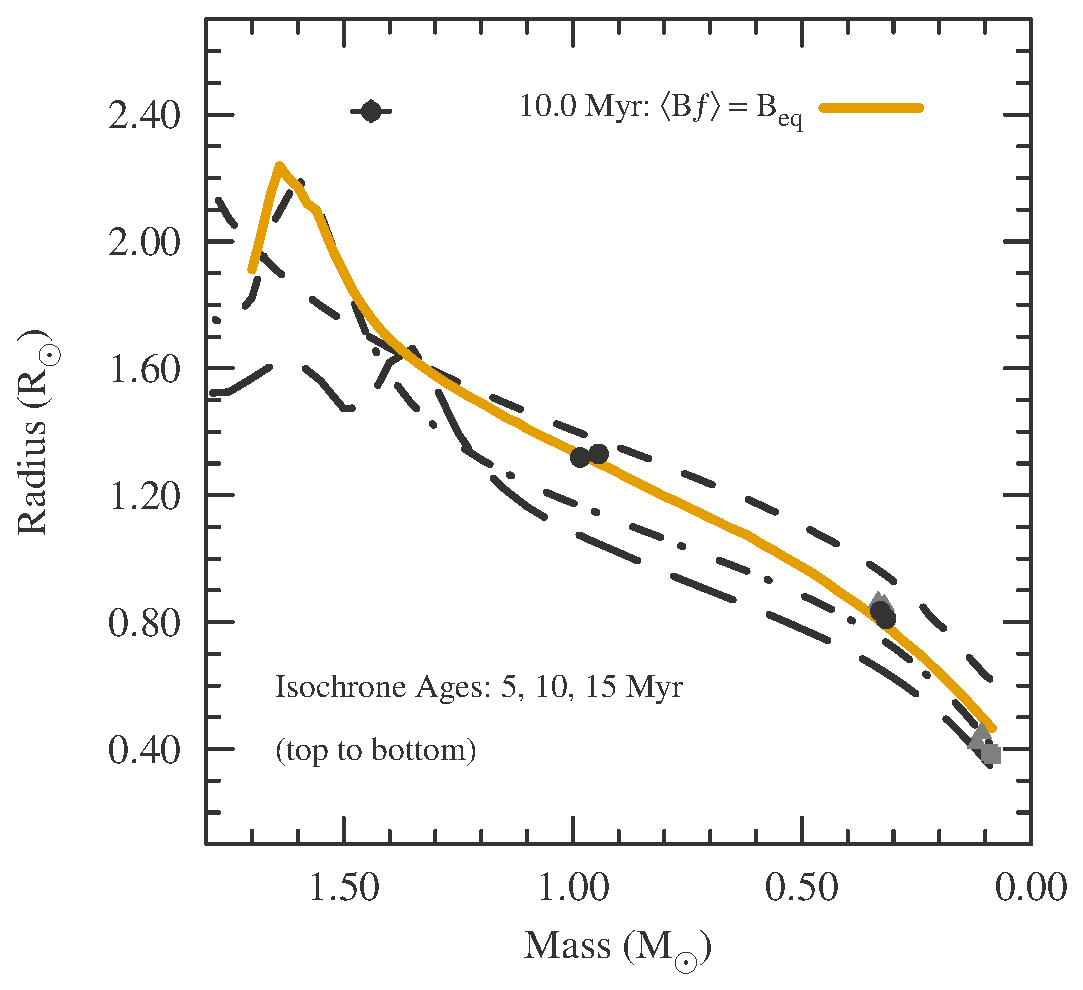
\includegraphics[width=0.45\linewidth]{./fig/USco_MR_diagram.eps}
	\caption{Caption.}
	\label{fig:usco}
\end{figure}

{\bf \large Project Description}

\textbf{P1. \emph{Dynamo-Generated Magnetic Fields throughout Early (sub)Stellar Evolution}} \\
Trace the temporal evolution of dynamo-generated magnetic fields. Explore how these properties depend on rotation, convection zone size, and stellar fundamental properties (surface temperature). Investigate the (1) topology of large-scale magnetic fields as a function of stellar mass, chemical composition, and age; (2) role of interior magnetic fields in governing stellar structure; and (3) the evolution of stellar activity cycles through polarity reversals of the large-scale field.
% Can we say anything about differential rotation, or is that assumed?

P1.1. --- \emph{Magnetic Fields in Surface Convection Zones of Low- and Intermediate-Mass Stars} \\
Straight 2D/3D models allow one to explore field properties as a function of stellar properties, but one loses temporal information. Strong magnetic fields are able to inhibit convective motions and delay contraction of young, pre-main-sequence stars. This means stellar rotation periods and convection zone sizes (core and surface) as a function of age differ between for stars with strong magnetic fields and those without. To model the feedback of the magnetic field on stellar properties over stellar evolutionary timescales (hundreds of thousands of years), simpler 1D stellar structure models are necessary. 

Core of project. Evolution of dynamo-generated magnetic fields in stellar convective envelopes. 
How is magnetic topology affected by rotation and the size of the convectie envelope/radiative 
core? How does the evolving topology influence the feedback on stellar structure? When and why
do stars transition from relatively "simple" axisymmetric, dipolar large-scale magnetic fields 
to predominantly non-axisymmetric, complex fields? Can we predict distribution of magnetic 
energy in $\mathcal{l}$-modes (spherical harmonic)? Trace temporal evolution of stellar magnetic
activity cycles and polarity reversals.

P1.2. --- \emph{Core Convection in the Presence of Magnetic Fields} \\
Investigate strength and topologies of magnetic fields in convection cores. Potential feedback
on stellar structure, suppression of overshoot? [IS THIS POSSIBLE?!] How does this affect the
approach to the MS? Long-term consequences for red giant asteroseismology.


P1.3. --- \emph{Magnetic Fields in Young Brown Dwarfs and Giant Planets} \\
Investigate how magnetic field generation is affected in cool, high pressure (degenerate) plasmas with
neutral outer layers. Is the thermal evolution of these objects affected by magnetic fields as with 
young stellar objects? Extract estimates of ohmic dissipation from dynamo models 
and account for extra heat in stellar models. [IS THIS POSSIBLE?!]

\textbf{P2. \emph{Starspots and Atmospheric Considerations}} \\
Improved treatment of surface boundary conditions through incorporation of detailed frequency-dependent radiative transfer. Seek to answer: How are surface boundary conditions affected by magnetic inhibition of convection, and how do they affect interior structure? How do starspots affect observational properties of young stars? '

Exploring the impact of starspots on observable properties (preliminary: Feiden \& Christophe, in prep). [NORDITA]
Including magnetic fields in stellar atmosphere models to better prescribe surface boundary conditions. [Uppsala]

\textbf{P3. \emph{Fundamental Properties of Young Single Stars}} \\
Confronting model predictions of young star properties as a function of age using a large number of stars characterized with spectro-bolometric techniques (CALYPSO) and young eclipsing binaries observed by Kepler/K2. [Hawaii; UT Austin]

Ages from the HRD rely on using fundamental stellar properties (radius, luminosity, Teff ) of a system of stars as comparison quantities. CMDs are incredibly useful tools for deriving ages, but as we?ve seen, are subject to several uncertainties. Using the HRD removes the uncertainty of converting model properties to colors and magnitudes. One is then interested to know whether stellar evolution models predict accurate fundamental properties for stars, thereby permitting accurate age determinations.

Previous investigations have found that young stellar models are unable to accurately predict effective temperatures and luminosities for stars at a given mass (e.g., ). These studies have focused on astrometric and eclipsing binaries (EBs), making it difficult to rule out whether binarity is playing a role in driving disagreements. Even wide binaries may be subject to subtle interactions that corrupt agreement with models. Recently, Stassun et al. (2014) showed that, while binarity in and of itself may not be a problem, model errors appear to be correlated with the presence of a tertiary companion. Triplicity among the same of EBs in Stassun et al. (2014) was well above 50\%, reducing the sample of potentially reliable comparisons to models and biasing our understanding of whether young models are accurate for predicting properties of single stars.

Therefore, we will create the first collection of single young benchmark stars, whose fun- damental properties will be measured with high precision (better than 5\% for young stars; Stassun et al. 2014). To derive stellar properties, collaborators Mann and Gaidos are obtain- ing ground-based, flux-calibrated spectra of bright K- and M-dwarfs in the nearby YMGs, the Pleiades, and Coma Berenices. Flux-calibrated spectra will be used to derive bolometric fluxes and effective temperatures, leading to empirical estimates of stellar radii. This technique was proven to be robust for assessing stellar evolution model reliability for main sequence field K- and M-dwarfs (Mann et al. 2015). Our current target sample contains 130 stars, twelve of which have already been observed and have preliminary properties.

Comparison of properties of benchmark stars to stellar models will be done using Bayesian inference to derive best fit model properties with uncertainties, as was performed in Mann et al. (2015) for main sequence stars. We will then explore how well models reproduce the observed data and whether there are any noticeable correlations with additional observables, such as magnetic activity indicators, inferred age, chemical composition, and the convective mixing length parameter. Since we are targeting stars that are members of known YMGs and clusters, we will also check for internal consistency, ensuring that models are yielding the same ages and distances to stars from a common group. If there are inconsistencies, we will attempt to characterize them in terms of observables and inferred stellar model parameters.

\textbf{P4. \emph{Homogeneous Ages for Young Stellar Associations}} \\
Deriving homogeneous ages for young stellar associations using available literature data. Provides constraints on a number of interesting astrophysical phenomena. [partially with UT Austin; Stockholm]

Informed by results obtained in work packages 1 and 2, we will bring together all of the information and try establish ages for young stellar systems that are consistent for different age measures, in both the HRD and CMDs. The age determinations will fold in all necessary ingredients, starting with a base set of standard young stellar models and exploring whether magnetic fields, starspots, or chemical composition are able to provide complete agreement for each system. We?ll explore the possibility that the appropriate mix of ingredients from work package 1 and other modified physics from work package 2 lead to consistent ages for all systems or if there are correlations among the mix of ingredients and stellar system parameters like age.

To avoid being entirely dependent on the success of WP01 and WP02, we will begin an initial effort characterizing how magnetic stellar models developed by GAF perform in terms of predicting consistent ages given different age indictors. Notably, consistency between high- and low-mass regions of CMDs and the HRD, as well as the lithium depletion boundary. We have preliminary results using a single eclipsing binary in Upper Sco (Kraus et al. 2015) that indicates magnetic models may provide favorable consistency between different mass regimes and between different age indicators for the binary alone (see Figure 2). We will therefore try to develop a more complete analysis of Upper Sco, including more archival data, and other nearby YMGs to determine the robustness of the solution. We will also provide our magnetic models to the community to permit additional independent efforts to evaluate the success or failures of these models.

Results of this exercise will be important, whether or not we are able to derive consistent ages or the different stellar systems. If we can derive consistent ages, then that will provide strong support for those derived ages, at least for the moment, which will become a powerful resource for the astronomical community. If we cannot, then we learn that there is yet something missing from models or that our initial hypothesis that low-mass stars are to blame for the systematic age differences observed in young stellar systems is incorrect.


Finally, this sub-project requires production of a grid of pre-main-sequence magnetic stellar models. Since the grid will be produced concurrently with the above studies, no additional time will be required. Local clusters at Uppsala will provide computational resources necessary and the PI is applying for time with SNIC, the Swedish high-performance computing center. All models, data products, and analysis tools will be made publicly available.

\clearpage

{\bf \large Significance}
\begin{itemize}
  \item Ages of Young Stars
  	\begin{itemize}
    	\item protoplanetary disk evolution timescales
    	\item giant planet formation timescales
    	\item star formation history, including time dependence of IMF
    	\item properties of directly imaged planets and brown dwarfs (mass distribution --> formation)
  	\end{itemize}
  \item Magnetic Field Evolution
  	\begin{itemize}
    	\item activity cycles --> astrobiology (stretch?)
    	\item angular momentum transport and stellar rotational evolution
    	\item accurate stellar properties
		\begin{itemize}
      		\item ages and masses of single stars
      		\item properties of transiting extrasolar planets
		\end{itemize}
     \end{itemize}
  \item Grid of Stellar Models
  	\begin{itemize}
		\item available to public
    	\item allows extensive testing of theory
	\end{itemize}
  \item Relevance for Next-Generation Surveys
\end{itemize}

{\bf \large Preliminary Results} \\
Feiden (2016, submitted). Identification of magnetic fields as culprit for age discrepancies.

Pilot study for the Sun (and low-mass star?).

Feiden \& Christophe (in preparation). Parametrized model of starspots.

Stars characterized for CALYPSO thus far.

{\bf \large Independent Line of Research}
\begin{itemize}
	\item Calibration of Low-Mass Young Stars and their Planetary Systems with Observations (CALYPSO): 
	second avenue of research is characterizing planets around young stars. 
    Feiden (projectledare) provides a comprehensive analysis of host stars using stellar models coupled 
    with Bayesian inference
    to give stellar mass, age, and distance estimates with realistic uncertainties.
	\item 4MOST Internal Working Group 7 -- Galactic Analysis Pipeline -- providing stellar
    structure and atmosphere code for self-consistent determination of atmospheric 
    parameters, mass, and ages for over 1 million stars.
    \item Zodiacal Exoplanets in Time (ZEIT).
\end{itemize}

{\bf \large International and National Collaborations}
\begin{itemize}
  	\item [Confirmed] Star formation group at UT Austin (Kraus, Rizzuto). Fundamental properties of young stars using B- through M-type EBs in young associations with Kepler/K2. Magnetic fields of young stars with IGRINS.
  	\item [Confirmed] CALYPSO: Calibration of Low-mass Young stars and their Planetary Systems with Observations (Mann [UT Austin], Gaidos [Hawaii], Ansdell [Hawaii]). Fundamental properties of bona fid\'{e} members of nearby young moving groups using "spectro-bolometric techniques."
  	\item [Pending] MDI/ZDI research group at ESO (Hussain, Lavail). Magnetic field topologies for young T-Tauri stars that can be compared against predictions from models in P1 with age information from P3.
  	\item [Pending] MDI/ZDI research group at Uppsala (Kochukhov, Ros\'{e}n). Magnetic field topologies for young solar analogs in young stellar associations.
  	\item [Confirmed] Open Cluster collaboration (Silvester, Landstreet). Magnetic field topologies for intermediate mass stars in several young stellar associations.
  	\item [Pending] Disk group at Stockholm (Janson)? Provide models to compute ages of directly imaged extrasolar planets and systems with circumstellar disks.
\end{itemize}


{\bf \large Other Grants}

\end{document}
